\documentclass{article}
\usepackage{geometry}
\geometry{hmargin = 2cm,vmargin = 2cm}
\usepackage[utf8]{inputenc}
\usepackage[T1]{fontenc}
\usepackage[table]{xcolor}
\usepackage{amssymb}
\usepackage{amsmath}
\usepackage{amsthm}
\usepackage{mathrsfs}
\usepackage{graphicx}
\usepackage{listings}
\usepackage{tikz}
\usetikzlibrary{arrows,positioning, calc}
\tikzstyle{vertex}=[draw,fill=white!15,circle,minimum size=20pt,inner sep=0pt]
\usepackage{color}
\definecolor{darkWhite}{rgb}{0.94,0.94,0.94}
\lstset{
  aboveskip=3mm,
  belowskip=-2mm,
  backgroundcolor=\color{darkWhite},
  basicstyle=\footnotesize,
  breakatwhitespace=false,
  breaklines=true,
  captionpos=b,
  commentstyle=\color{red},
  deletekeywords={...},
  escapeinside={\%*}{*)},
  extendedchars=true,
  framexleftmargin=16pt,
  framextopmargin=3pt,
  framexbottommargin=6pt,
  frame=tb,
  keepspaces=true,
  keywordstyle=\color{blue},
  language=python,
  literate=
  {²}{{\textsuperscript{2}}}1
  {⁴}{{\textsuperscript{4}}}1
  {⁶}{{\textsuperscript{6}}}1
  {⁸}{{\textsuperscript{8}}}1
  {€}{{\euro{}}}1
  {é}{{\'e}}1
  {è}{{\`{e}}}1
  {ê}{{\^{e}}}1
  {ë}{{\¨{e}}}1
  {É}{{\'{E}}}1
  {Ê}{{\^{E}}}1
  {û}{{\^{u}}}1
  {ù}{{\`{u}}}1
  {â}{{\^{a}}}1
  {à}{{\`{a}}}1
  {á}{{\'{a}}}1
  {ã}{{\~{a}}}1
  {Á}{{\'{A}}}1
  {Â}{{\^{A}}}1
  {Ã}{{\~{A}}}1
  {ç}{{\c{c}}}1
  {Ç}{{\c{C}}}1
  {õ}{{\~{o}}}1
  {ó}{{\'{o}}}1
  {ô}{{\^{o}}}1
  {Õ}{{\~{O}}}1
  {Ó}{{\'{O}}}1
  {Ô}{{\^{O}}}1
  {î}{{\^{i}}}1
  {Î}{{\^{I}}}1
  {í}{{\'{i}}}1
  {Í}{{\~{Í}}}1,
  morekeywords={*,...},
  numbers=left,
  numbersep=10pt,
  numberstyle=\tiny\color{black},
  rulecolor=\color{black},
  showspaces=false,
  showstringspaces=false,
  showtabs=false,
  stepnumber=1,
  stringstyle=\color{gray},
  tabsize=4,
  title=\lstname,
}
%pour la compilation minted : C:\Users\Serge\Anaconda3\pkgs\pygments-2.2.0-py37_0\Scripts à ajouter en PATH et 
%remplacer pdflatex -synctex=1 -interaction=nonstopmode %.tex
%par pdflatex -synctex=1 -interaction=nonstopmode --shell-escape %.tex
\title{Quadtree}
\author{Tout le monde}
\begin{document}
\maketitle

\newpage

\tableofcontents

\section{Implémentation : comparaison entre structure récursive et représentation en liste}
\subsection{Structure récursive}
Une représentation qui semble la plus naturelle est d'implémenter une structure avec auto-référence. En effet en s'inspirant de la définition inductive on peut voir un arbre binaire comme une structure contenant essentiellement 3 champs : une clef et deux arbres binaires, ses sous-arbres gauche et droit. 
En terme d'implémentation cela dépend du langage utilisé. \\
 En C cela passera par la création d'un type spécifique arbre avec en variable des pointeurs vers des variables de ce même type, en plus d'une variable clef de type entier par exemple. \\
En suivant le paradigme de la programmation objet, on créé une classe arbre ayant deux attributs de type arbre en plus de l'attribut clef (et d'autres attributs si nécessaires). La souplesse de Python sur les types rend la création de la classe particulièrement aisée mais il faudra être vigilant sur l'utilisation. 
On pourra déclarer la classe comme ceci :

\begin{lstlisting}
class ArbreBinaire():
    def __init__(self,clef,gauche = None ,droite = None):
        """ Anything x ArbreBinaire x ArbreBinaire -> ArbreBinaire
        Constructeur d'arbre"""
        self.clef = clef
        self.gauche = gauche
        self.droite = droite
\end{lstlisting}

Exemple d'instanciation :

\begin{lstlisting}
Feuille1 = ArbreBinaire(1)
Feuille2 = ArbreBinaire(2)
Arbre = ArbreBinaire(3,Feuille1,Feuille2)
\end{lstlisting}

L'arbre créé est :
\begin{center}
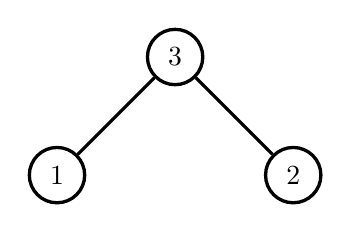
\begin{tikzpicture}[very thick,level/.style={sibling distance=30mm/#1}]
\node [vertex] (r){$3$}
  child {
    node [vertex] (a) {$1$}
   }
   child {
    node [vertex] (a) {$2$}
   }
   
   ;
\end{tikzpicture}
\end{center}

\subsection{Liste}
On peut aussi représenter l'arbre sous forme de liste. L'idée est d'avoir la racine au début de la liste, le fils gauche à l'index 1, le fils droite à l'index 2 et ainsi de suite. Pour un nœud à l'indice i, on trouve son fils gauche à l'indice 2i de la liste, et le droit à l'indice 2i+1. 
On peut donc également retrouver le père d'un nœud facilement : pour un nœud d'index i, le père est à l'index $\lfloor \frac{i-1}{2} \rfloor$ (on prend la partie entière dans la division par 2).
On fera attention à ne pas sauter les nœuds vides, il faut bien les représenter dans la liste par un caractère spécial en fonction de ce que l'arbre contient comme type de donnée. Par exemple mettre False pour un arbre contenant des entiers éventuellement nuls n'est pas une bonne solution, le test False == 0 renvoyant true en Python (et beaucoup d'autres langages).
Par exemple l'arbre suivant :

\begin{center}
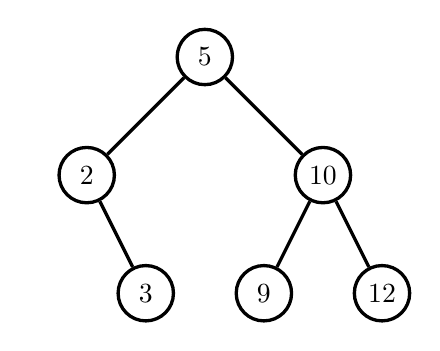
\begin{tikzpicture}[very thick,level/.style={sibling distance=30mm/#1}]
\node [vertex] {$5$}
  child {
    node [vertex]  {$2$}
    child{edge from parent[draw=none]}
    child{node [vertex] {$3$}}
   }
   child {
    node [vertex] {$10$}
    child{node [vertex] {$9$}}	
    child{node [vertex] {$12$}}
   };
\end{tikzpicture}
\end{center}

sera représenté par la liste :
$[5,2,10,"vide",3,9,12]$

Remarquons qu'idéalement il faut utiliser une structure qui combine les avantages de la liste chaînée et des tableaux : nous avons besoins d'accéder à aux éléments à une position précise en temps constant si possible, mais la structure doit être de taille flexible pour l'agrandir ou la réduire. 
\subsection{Comparaison}
\subsubsection{Avantages et inconvénients}
\paragraph*{}
Pour la structure récursive :
\begin{itemize}
\item[•]
Lisibilité du code.
\item[•]
Gain mémoire pour les arbres avec des nœuds vides : on n'insère que les nœuds non vide dans l'abre.
\item[•]
Plus grande souplesse dans le type de donnée représentée dans le nœud.
\end{itemize}
\paragraph*{}
Pour la représentation en liste :
\begin{itemize}
\item[•]
Gain de mémoire pour les arbres pleins ou parfait.
\item[•]
Simplicité de la mise en place, notamment pour les langages implémentant déjà une structure de liste / tableau (en Python on dispose par exemple déjà des primitives append, pop, len etc).
\item[•]
Accès immédiat au parent.
\end{itemize}
Les inconvénients se déduisent des avantages : pour la structure récursive elle est plus lourde à mettre en place, ça peut être lourd en mémoire pour des arbres pleins.
Pour la liste, le code sera peut être moins lisible et surtout on gâche de la mémoire lorsque l'arbre contient des nœuds vide. 

Dans certains cas la liste est particulièrement appropriée par exemple pour la représentation des tas (arbre binaire parfait sur un ensemble totalement ordonnée où les chemins de la racine vers les feuilles est toujours croissant), utilisée dans le tri par tas où le but est d'ordonner une liste. 
\end{document}
